\section*{\fs{12}Zapytanie z podzapytaniem w Select}
\par{
\fs{12}
\subsection*{\fs{12} Osoba z największą ilością pobytów w szpitalu}


\listsinglespacing{
\fs{12}
\begin{lstlisting}[frame=single,language=SQL,]
Select TOP 1  imie,nazwisko,
(select COUNT(*) from Pobyt where Pacjent.pesel=Pobyt.pesel) as [Ilość Pobytów w Szpitalu]
from Pacjent 
order by [Ilość Pobytów w Szpitalu] Desc

\end{lstlisting}
\begin{figure}[h!]
    \centering
   \scalebox{.85}{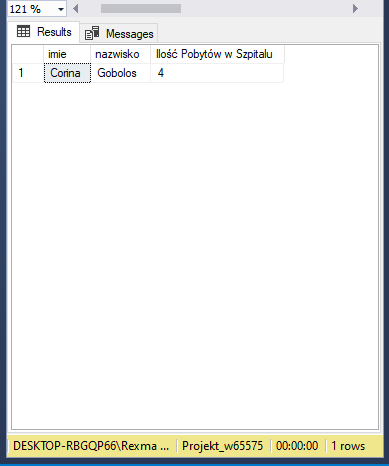
\includegraphics{Images/Zadanie3/P4/Z16a.png}}
    \caption{Wynik Zapytania}
    \label{fig:my_label}
\end{figure}
}
\begin{figure}[h!]
    \centering
   \scalebox{.60}{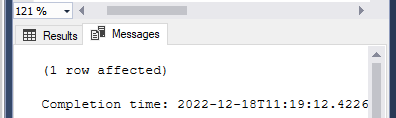
\includegraphics{Images/Zadanie3/P4/Z16b.png}}
    \caption{Wynik Zapytania}
    \label{fig:my_label}
\end{figure}
\newpage
\subsection*{\fs{12} Imie i Nazwisko pacjeta i nazwa oddziału na jaki został ostatnio przyjęty}

\listsinglespacing{
\fs{12}
\begin{lstlisting}[frame=single,language=SQL,]
Select Imie, nazwisko , 
(Select Top 1  O.Nazwa 
from Pobyt as P inner join 
Oddział as O 
on P.oddział=O.id_oddziału 
where Pacjent.pesel=P.pesel
order by data_przyjecia desc 
)
from Pacjent

\end{lstlisting}
\begin{figure}[h!]
    \centering
   \scalebox{.85}{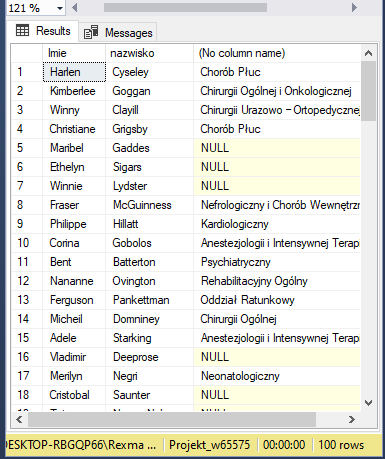
\includegraphics{Images/Zadanie3/P4/Z17a.png}}
    \caption{Wynik Zapytania}
    \label{fig:my_label}
\end{figure}
}

\begin{figure}[h!]
    \centering
   \scalebox{.60}{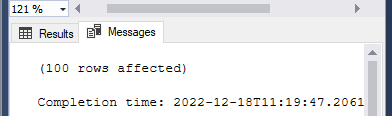
\includegraphics{Images/Zadanie3/P4/Z17b.png}}
    \caption{Wynik Zapytania}
    \label{fig:my_label}
\end{figure}
\newpage
\clearpage
\subsection*{\fs{12} Specjalizacje pracowników}
\listsinglespacing{
\fs{12}
\begin{lstlisting}[frame=single,language=SQL,]
Select Imie, Nazwisko, (Select top 1 nazwa from Pracownicy_specjalizacje
inner join Specjalizacje on 
Pracownicy_specjalizacje.id_specjalizacji=Specjalizacje.id_specjalizacji 
where Pracownicy.id_pracownika=Pracownicy_specjalizacje.[id_pracownika])
From Pracownicy

-- wersja z wykorzystaniem with

with spec as (
Select  nazwa,Pracownicy.id_pracownika as idp
from Pracownicy_specjalizacje 
inner join Specjalizacje 
on Pracownicy_specjalizacje.id_specjalizacji=Specjalizacje.id_specjalizacji 
inner join Pracownicy
on Pracownicy.id_pracownika=Pracownicy_specjalizacje.id_pracownika
where Pracownicy.id_pracownika=Pracownicy_specjalizacje.[id_pracownika]
)
Select  imie ,nazwisko,spec.nazwa
from Pracownicy
inner join spec
on spec.idp=Pracownicy.id_pracownika
where spec.nazwa is not null 

\end{lstlisting}
\begin{figure}[h!]
    \centering
   \scalebox{.85}{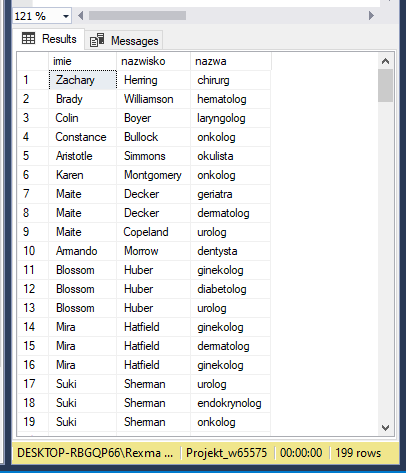
\includegraphics{Images/Zadanie3/P4/Z18a.png}}
    \caption{Wynik Zapytania}
    \label{fig:my_label}
\end{figure}
}
\begin{figure}[h!]
    \centering
   \scalebox{.60}{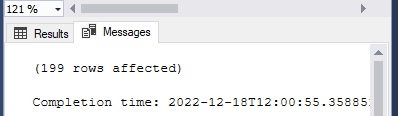
\includegraphics{Images/Zadanie3/P4/Z18b.png}}
    \caption{Wynik Zapytania}
    \label{fig:my_label}
\end{figure}
\newpage